%%%%%%%%%%%%%%%%%%%%%%%%%%%%%%%%%%%%%%%%%
% University/School Laboratory Report
% LaTeX Template
% Version 3.1 (25/3/14)
%
% This template has been downloaded from:
% http://www.LaTeXTemplates.com
%
% Original author:
% Linux and Unix Users Group at Virginia Tech Wiki 
% (https://vtluug.org/wiki/Example_LaTeX_chem_lab_report)
%
% License:
% CC BY-NC-SA 3.0 (http://creativecommons.org/licenses/by-nc-sa/3.0/)
%
%%%%%%%%%%%%%%%%%%%%%%%%%%%%%%%%%%%%%%%%%

%----------------------------------------------------------------------------------------
%	PACKAGES AND DOCUMENT CONFIGURATIONS
%----------------------------------------------------------------------------------------

\documentclass{article}


\usepackage{listings}
\lstset{
language=Swift,
basicstyle=\small\ttfamily,
columns=flexible,
breaklines=true,
breakatwhitespace=false,
literate={à}{{\'a}}1 {è}{{\'e}}1 {ò}{{\'o}}1 {ù}{{\'u}}1 {ì}{{\'\i}}1,
}

\usepackage[T1]{fontenc}
\usepackage[italian]{babel}
\usepackage[utf8]{inputenc}

\usepackage{siunitx} 						% Provides the \SI{}{} and \si{} command for typesetting SI units
\usepackage{graphicx}						% Required for the inclusion of images
\usepackage{natbib} 							% Required to change bibliography style to APA
\usepackage{amsmath}						% Required for some math elements 

\setlength\parindent{0pt} 					% Removes all indentation from paragraphs

\renewcommand{\labelenumi}{\alph{enumi}.} % Make numbering in the enumerate environment by letter rather than number (e.g. section 6)

%\usepackage{times} % Uncomment to use the Times New Roman font

%----------------------------------------------------------------------------------------
%	DOCUMENT INFORMATION
%----------------------------------------------------------------------------------------

\title{Laboratorio di Applicazioni Mobili\\Informatica, Università di Bologna} % Title

\author{Matteo Celani} % Author name

\date{2019-2020} % Date for the report

\begin{document}

\maketitle % Insert the title, author and date

\begin{center}
\begin{tabular}{l r}
Docente: 					& Luciano Bononi \\ 
Docente: 					& Federico Montori  \\ 
\medskip
Tutor didattico: 		& Luca Sciullo \\ 
Mail: 							& matteo.celani@studio.unibo.it \\
\bigskip
Matricola: 					& 0000804303 \\
GitHub: 					&www.github.com/matteocelani/PersonalHealthMonitor\\
\end{tabular}
\end{center}

%----------------------------------------------------------------------------------------
%	INDICE
%----------------------------------------------------------------------------------------
\newpage
\tableofcontents

\newpage
\section{Personal health monitor}

Nel seguente progetto lo studente è tenuto a implementare un'applicazione interattiva per tenere traccia delle informazioni personali sulla propria salute da salvare nei report giornalieri. In particolare, l'applicazione dovrebbe essere in grado di gestire i report all'interno di un calendario, inviare notifiche e tracciare i dati in base a filtri specifici.

\subsection{Creare e modificare report}

L'applicazione deve essere in grado di creare, modificare ed eliminare i rapporti sulla salute. I rapporti sulla salute sono riassunti delle informazioni sulla salute tracciati dall'utente che devono essere salvati ogni volta che l'utente ritiene che sia una buona idea e almeno una volta al giorno. Ogni rapporto deve includere un numero minimo di due informazioni relative alla salute dell'utente (ad es. Temperatura corporea, pressione sanguigna, indice glicemico, ecc.). Ogni informazione ha un'importanza, cioè un indice che specifica il livello di attenzione che richiede tale parametro (da 1 a 5) e ogni rapporto ha una nota opzionale che può essere riempita con informazioni ausiliarie. I report vengono archiviati dall'applicazione (si consiglia vivamente di utilizzare un database) e deve esserci la possibilità di mostrare report su base giornaliera, come ad esempio all'interno di un calendario. Nel caso di più report per lo stesso giorno, è necessario creare un report di riepilogo, in cui le informazioni sulla salute sono la media di tutti i dati raccolti di quel giorno. Ci deve essere anche la possibilità di visualizzare i report in base ad alcuni filtri (ad esempio, solo i report con importanza impostata su 5).

\subsection{Notifiche}

L'applicazione deve avvisare l'utente se non ha ancora inserito un rapporto per quel giorno. In questo caso, l'utente può eseguire le seguenti azioni: rinviare il promemoria (in tal caso all'utente verrà richiesta un'altra ora e data dello stesso giorno) o aprire direttamente dall'interno della notifica il modulo per la compilazione del rapporto. Il tempo in cui la notifica viene inviata dall'applicazione può essere impostato dall'utente da una pagina delle impostazioni. L'applicazione deve inoltre informare l'utente se la media dei dati raccolti per un'informazione - con importanza maggiore di 3 - in un determinato periodo di tempo ha superato una soglia predefinita. L'utente può personalizzare i parametri precedenti da una pagina delle impostazioni, ovvero può decidere quali informazioni devono essere monitorate, per quanto tempo e quale soglia non deve essere raggiunta.

\subsection{Grafici}

L'applicazione dovrebbe essere in grado di raccogliere statistiche sull'utilizzo che visualizzano almeno due grafici di qualsiasi tipo (grafico a torta, diagramma a riquadri, istogramma, grafico a linee, ecc.) Che mostrano dati utili (ad esempio la variazione di informazioni sanitarie nell'arco di una settimana, la variazione di il numero di rapporti raccolti ogni giorno, ecc.).

%----------------------------------------------------------------------------------------
%	Introduzione app
%----------------------------------------------------------------------------------------

\newpage
\section{HealtMonitor per iOS}

Questa versione di HealtMonitor è stata pensata e sviluppa per \textbf{iOS 13} usando \textbf{Swift 5} su \textbf{xCode 11}.

L'app è divisa in 3 sezioni principali richiamate nel ContentView.swift : 
\begin{itemize}
  \item \texttt{Summary()}
  \item \texttt{CalendarTab()}
  \item \texttt{AddReport() }
\end{itemize}

Ogni view viene invocata tramite la TabView, in \textit{"Riepilogo"} abbiamo i grafici dei valori inseriti e la lista di tutti i report, in \textit{"Calendario"} abbiamo un calendario organizzato per mesi dove si può controllare i giorni in cui si è inserito il report, infine possiamo aggiungere un nuovo report nell'ultima tab \textit{"Nuovo"}.

\medskip

\begin{figure}[htp]

\centering
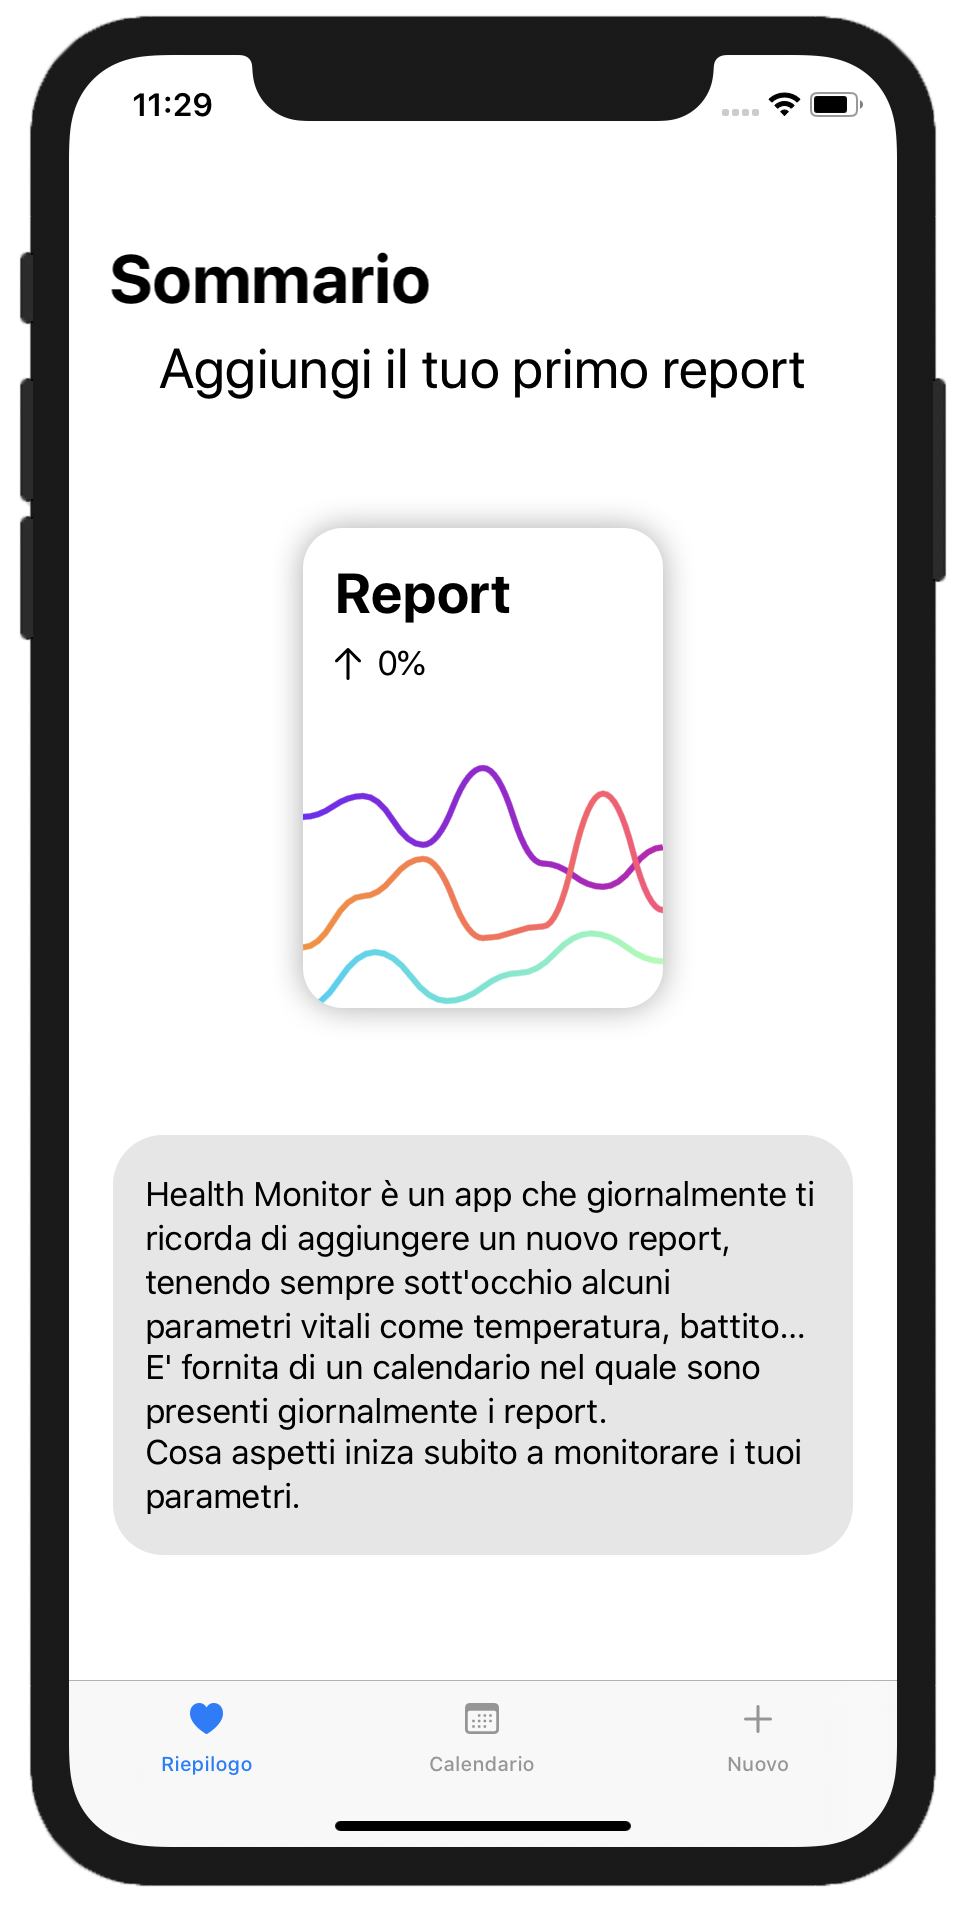
\includegraphics[width=.3\textwidth]{img/riepilogo_iniziale.png}\hfill
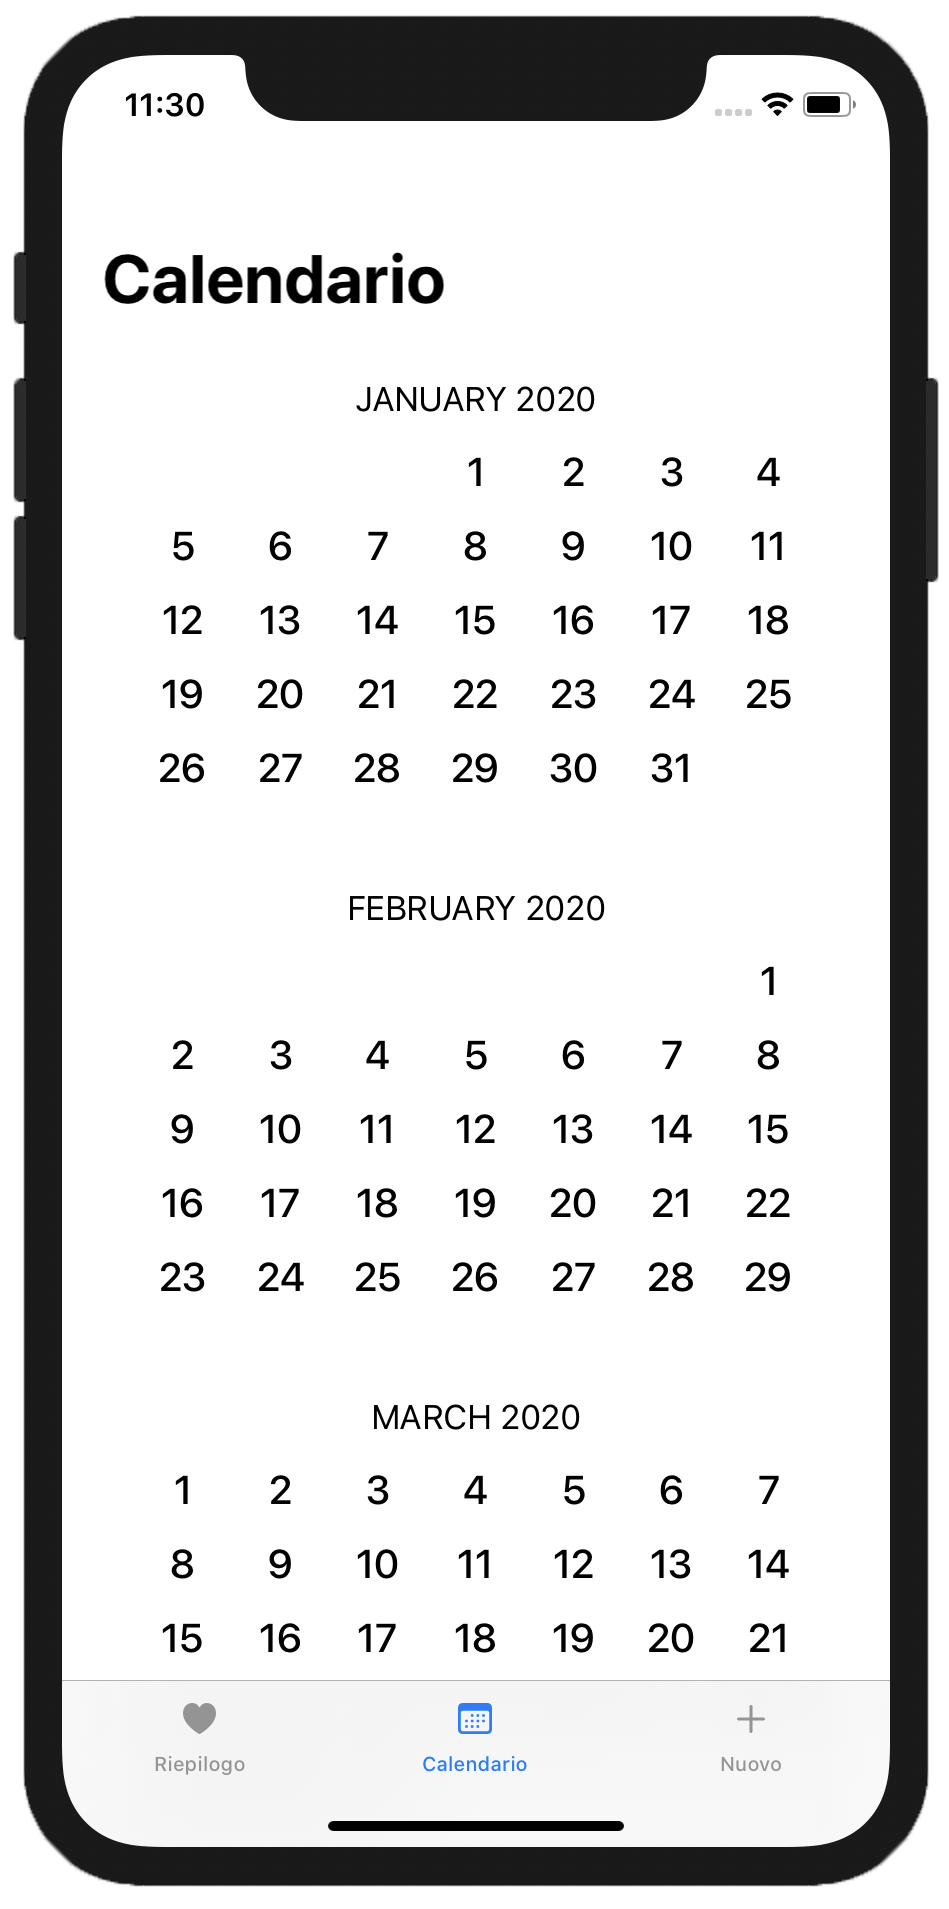
\includegraphics[width=.3\textwidth]{img/calendario_iniziale.png}\hfill
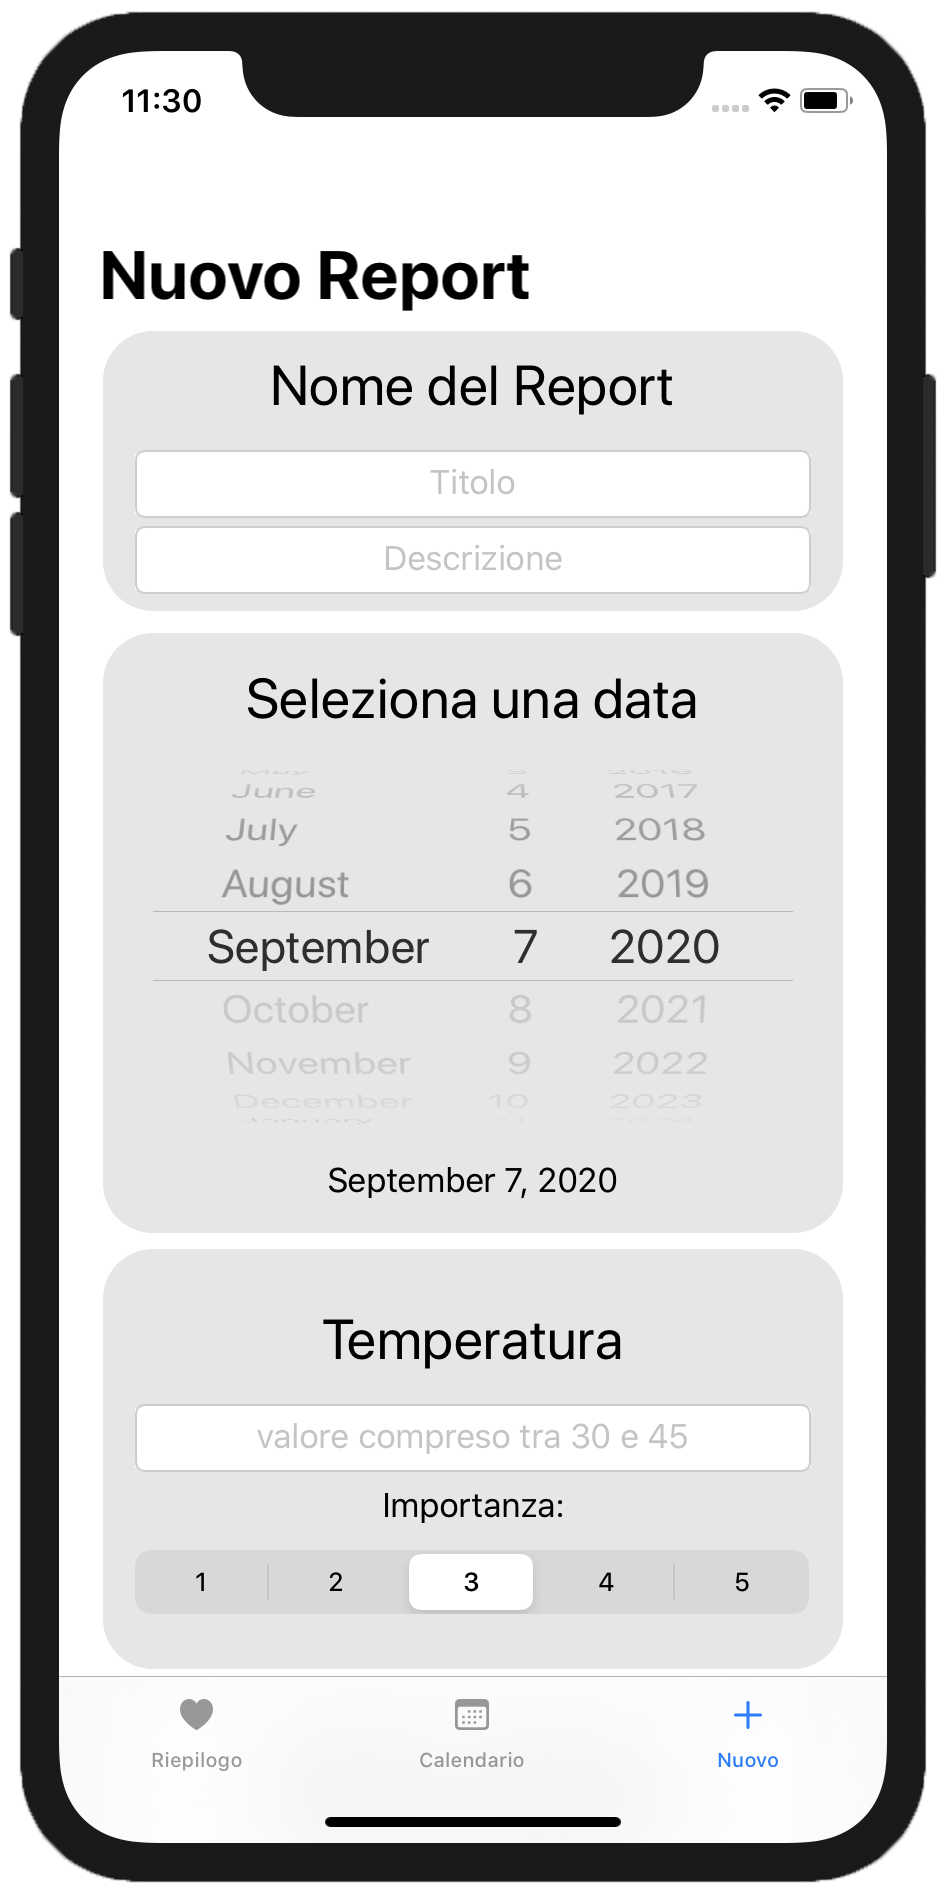
\includegraphics[width=.3\textwidth]{img/nuovo_iniziale.png}

\caption{Schermate Iniziali}
\label{fig:figure3}

\end{figure}

%----------------------------------------------------------------------------------------
%	Riepilogo
%----------------------------------------------------------------------------------------

\newpage
\section{Riepilogo}

In riepilogo vengono generati i grafici relativi ai dati inseriti giorno per giorno inoltre è presenta una lista dove si possono consultare tutti i Report. I report possono essere visualizzati tramite alcuni filtri, possono essere modificati ed eliminati.\\
Se non è presente nessun dato viene caricata una schermata iniziale di benvenuto. 

\begin{figure}[htp]

\centering
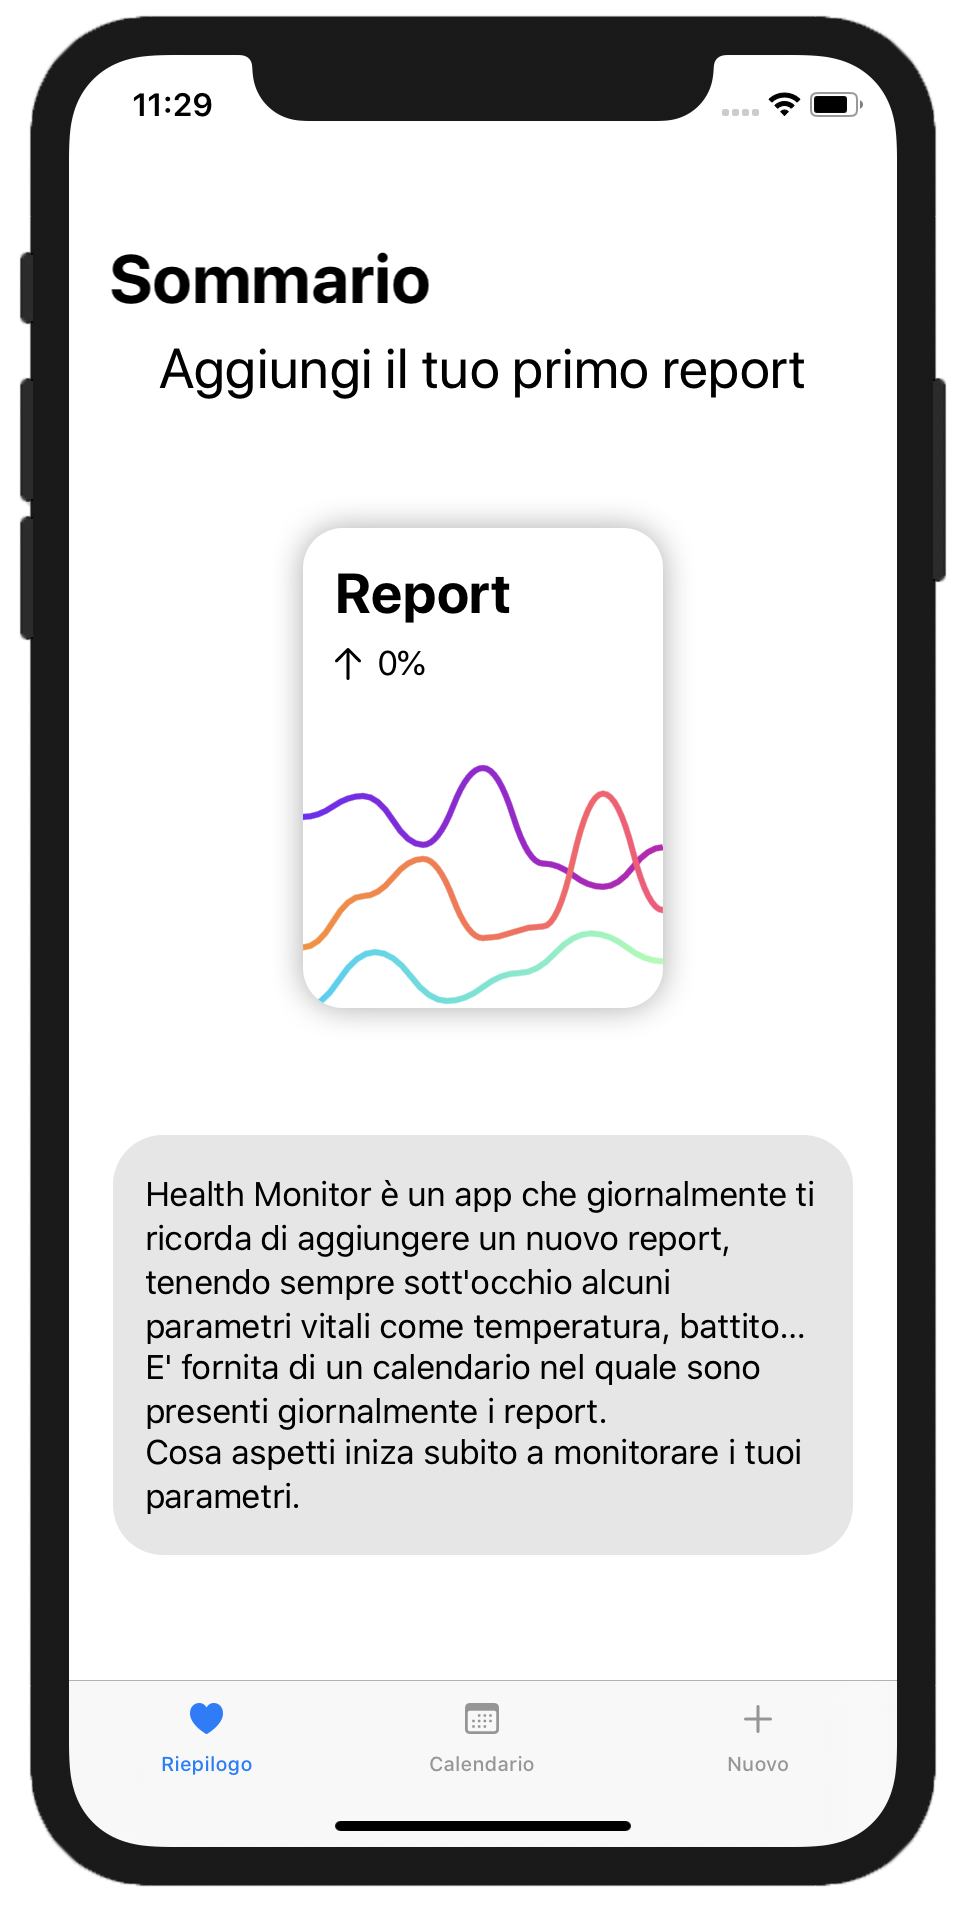
\includegraphics[width=.3\textwidth]{img/riepilogo_iniziale.png}

\caption{Schermata di benvenuto}
\label{fig:figure3}
\end{figure}

\subsection{Grafici}

Quando si inseriscono i dati, si iniziano a generare 4 grafici uno per ogni valore presente nel Report.\\
I grafici generati usando un pacchetto Swift dal nome \textbf{\textit{"SwiftUICharts"}}, esso permette di generare grafici, prendendo in input array di dati di tipo Double. Si è reso necessario trasformare i \textbf{Core Data} in array ordinati con tutti gli elementi di tipo Double tramite 4 semplici funzioni: \texttt{reportTempArray()}, \texttt{reportHeaArray()}, \texttt{reportGlyArray()}, \texttt{reportBreArray()}.\\
I valori dei grafici sono ordinati per data, basta trascinare il dito sopra al grafico per visualizzarli. 

\begin{figure}[htp]

\centering
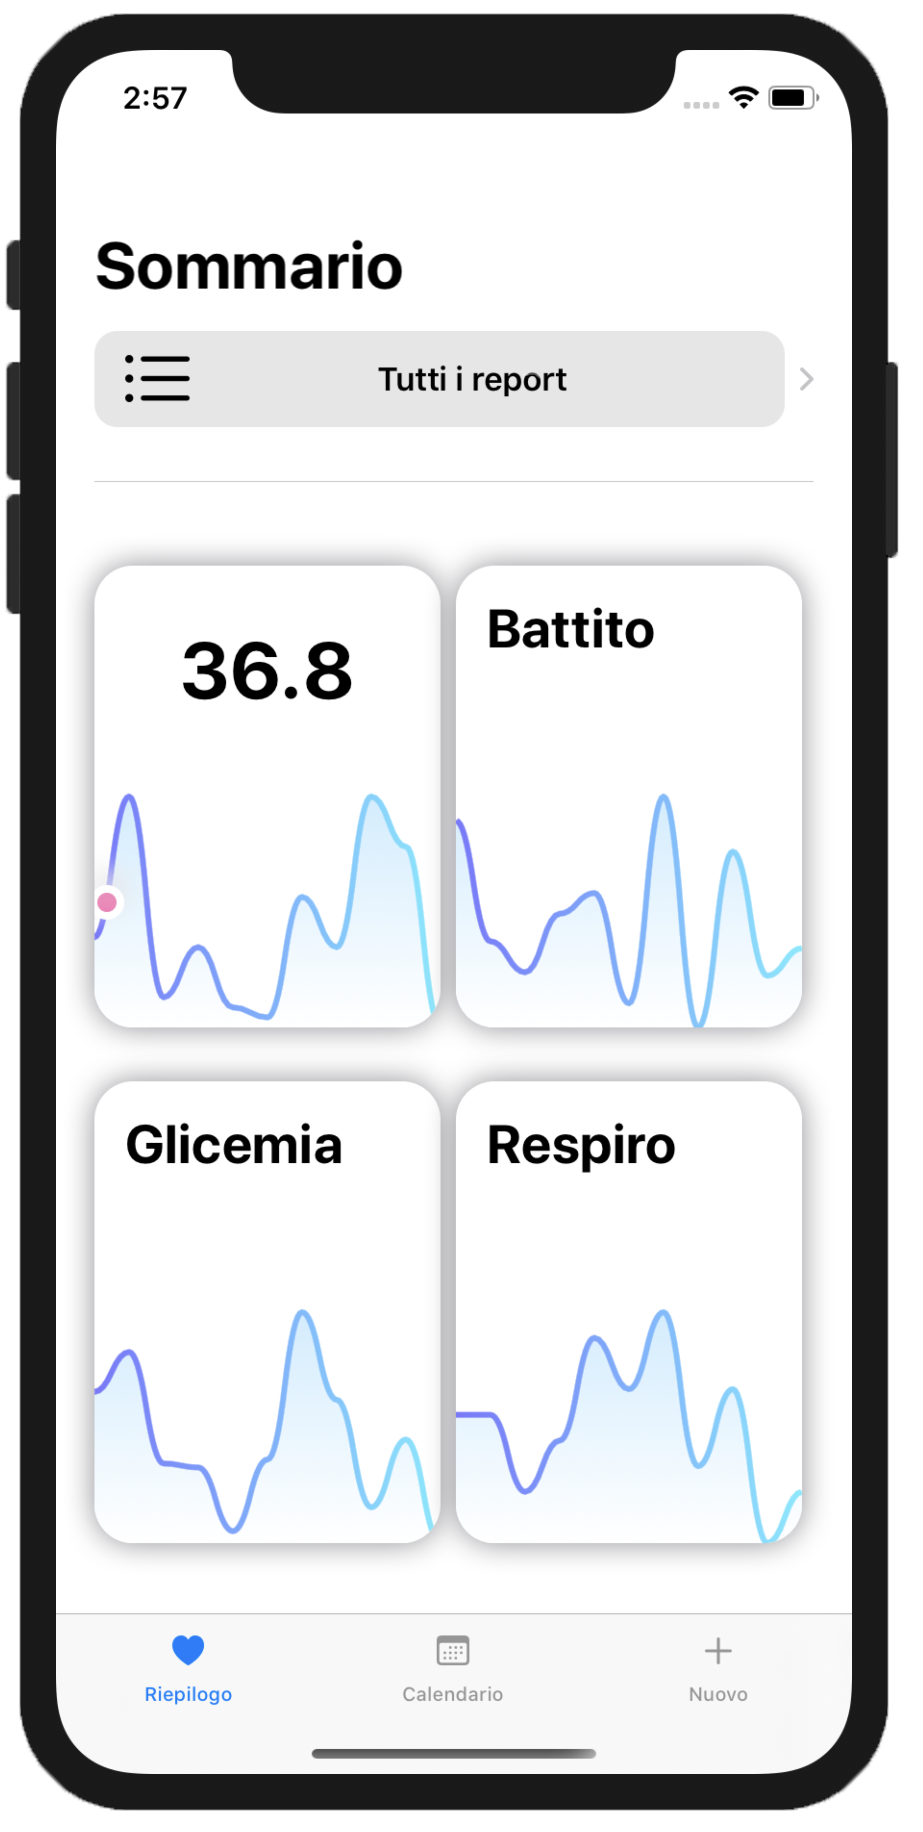
\includegraphics[width=.3\textwidth]{img/grafico1.png}\hfill
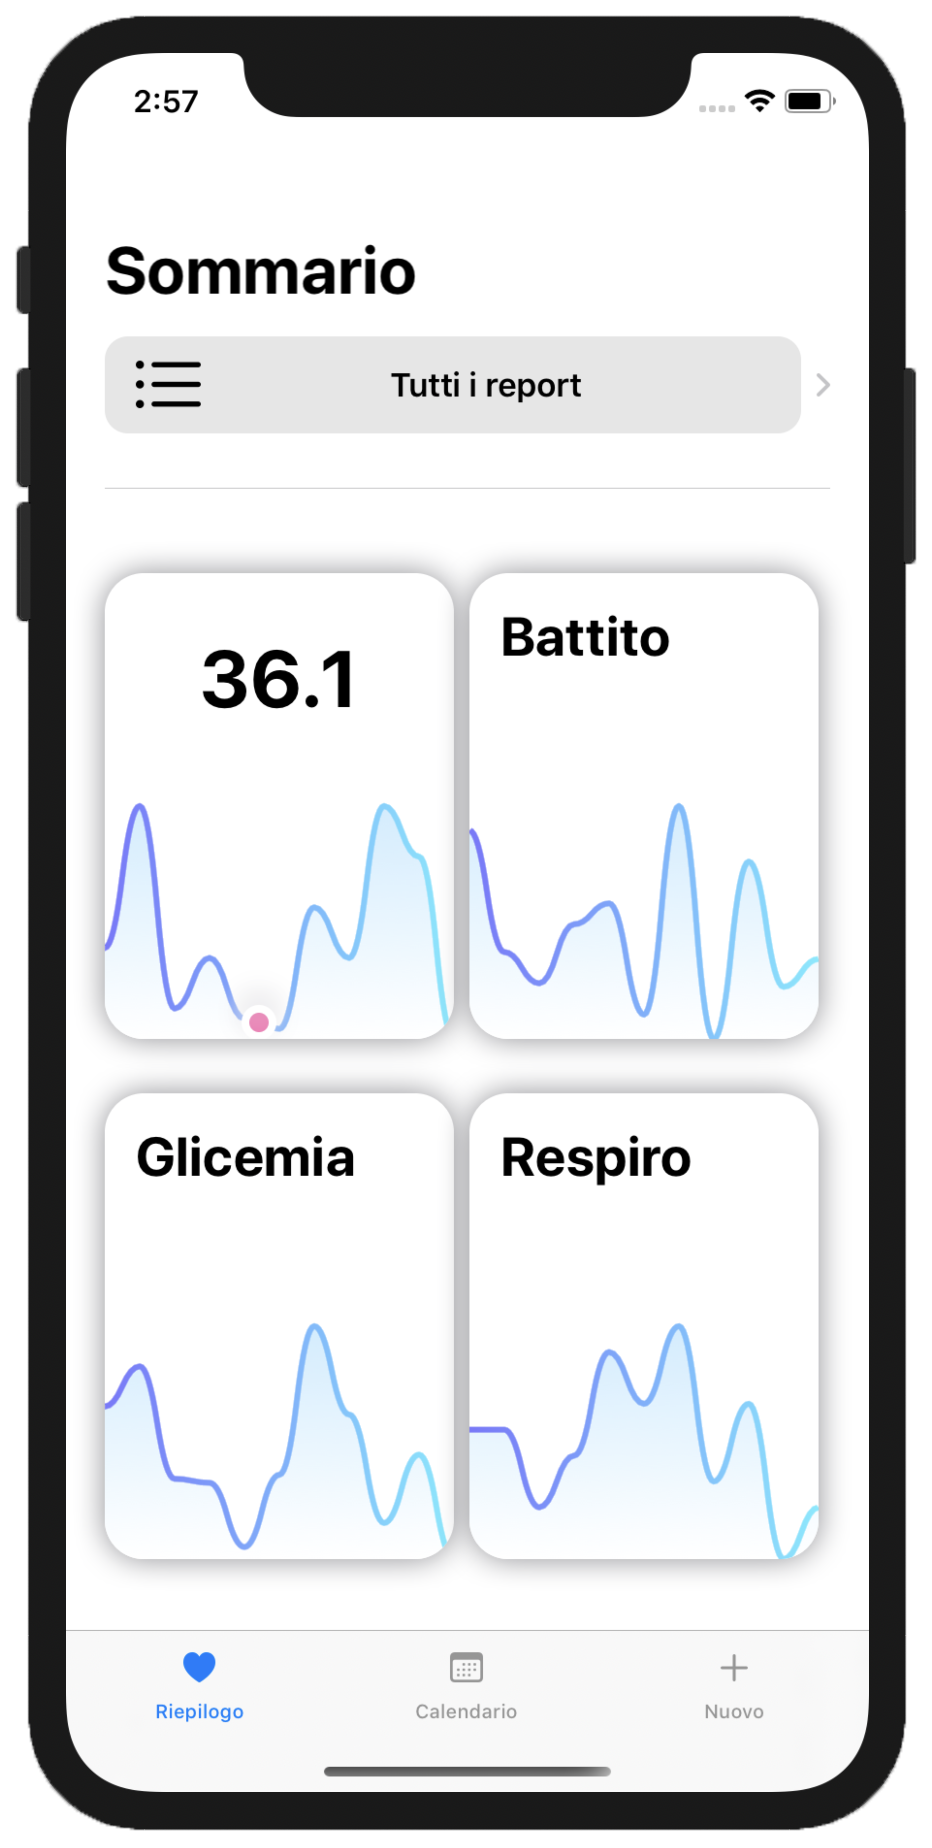
\includegraphics[width=.3\textwidth]{img/grafico2.png}\hfill
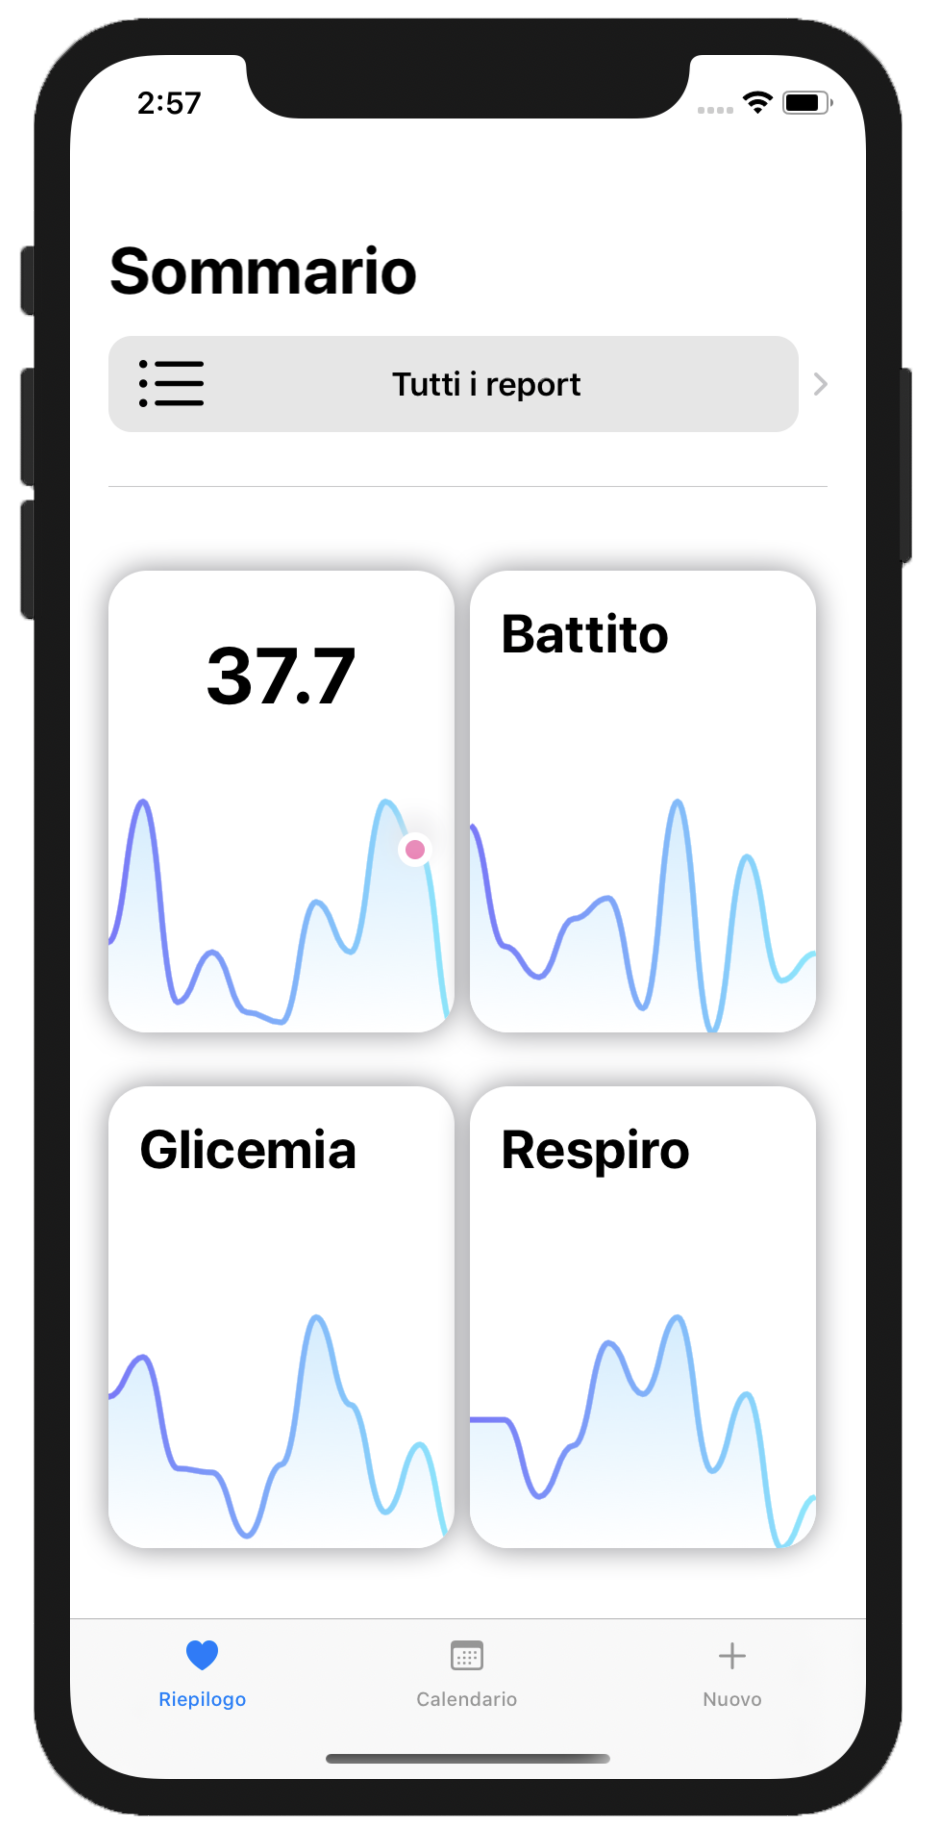
\includegraphics[width=.3\textwidth]{img/grafico3.png}

\caption{Grafici con valori}
\label{fig:figure3}

\end{figure}

\newpage

\subsection{Tutti i grafici}

\begin{lstlisting}
NavigationLink(destination: AllReport()) {
	ListView(content: AnyView(
		HStack {
			Image(systemName: "list.bullet").font(.largeTitle)
			Spacer()
			Text("Tutti i report")
			.font(.headline)
			 Spacer()
		}
	))
}

\end{lstlisting}

\begin{figure}[htp]

\centering
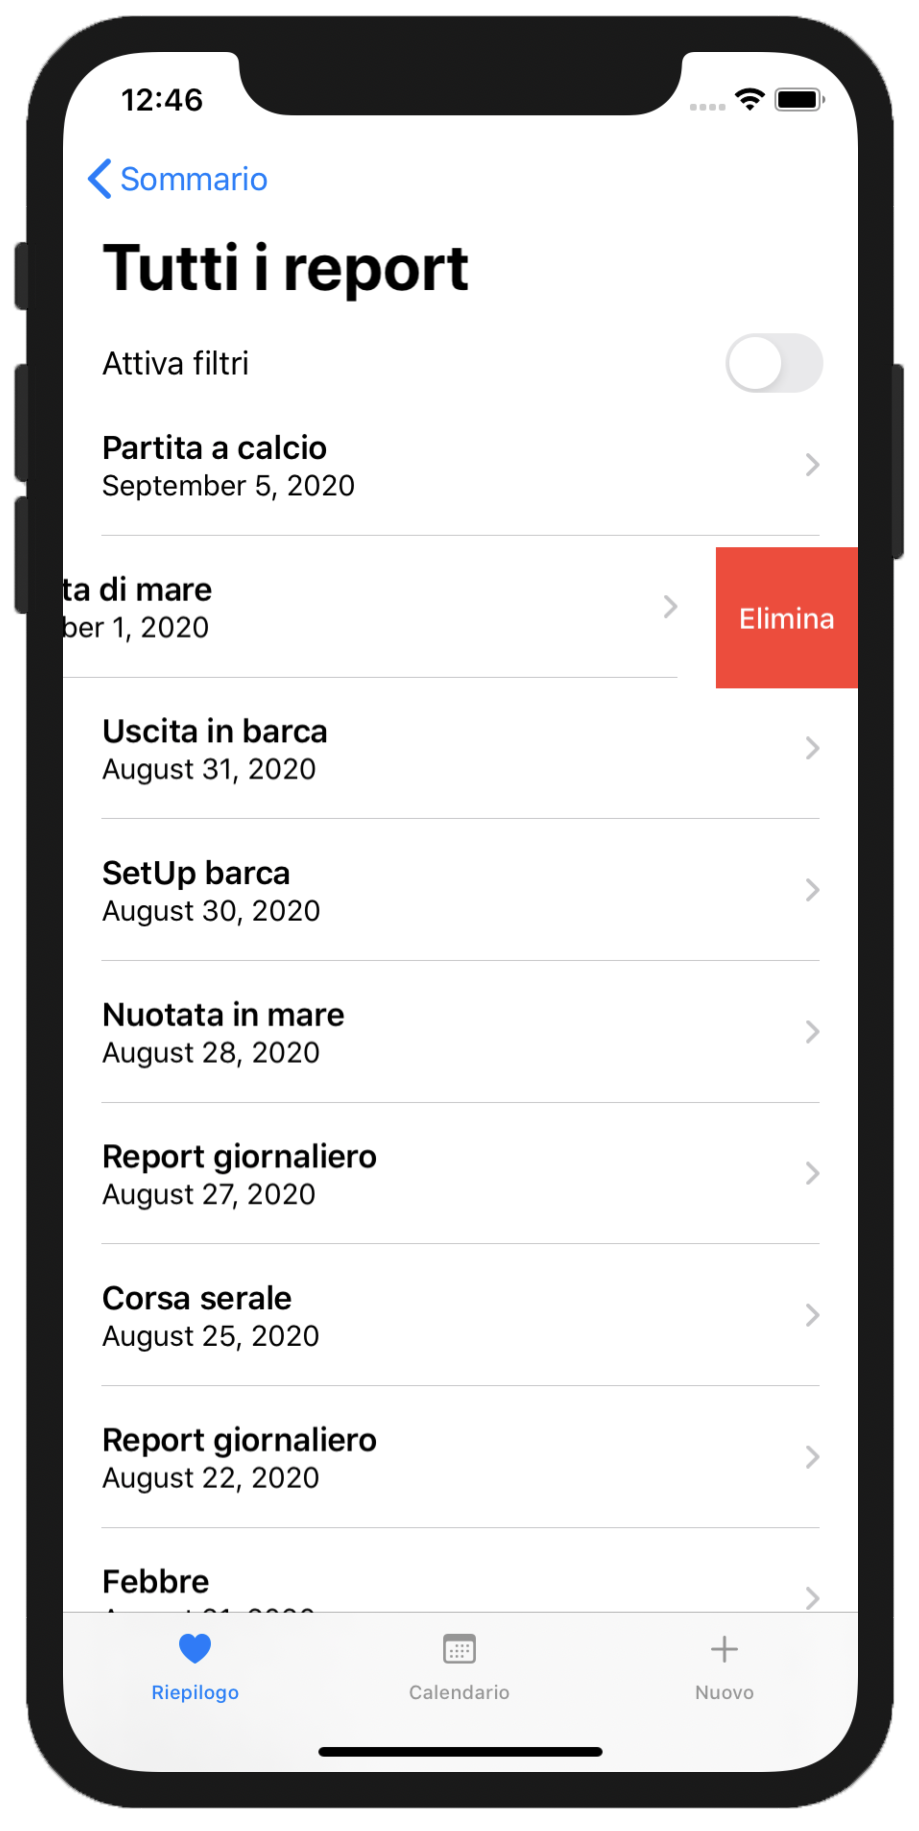
\includegraphics[width=.3\textwidth]{img/tutti1.png}\hfill
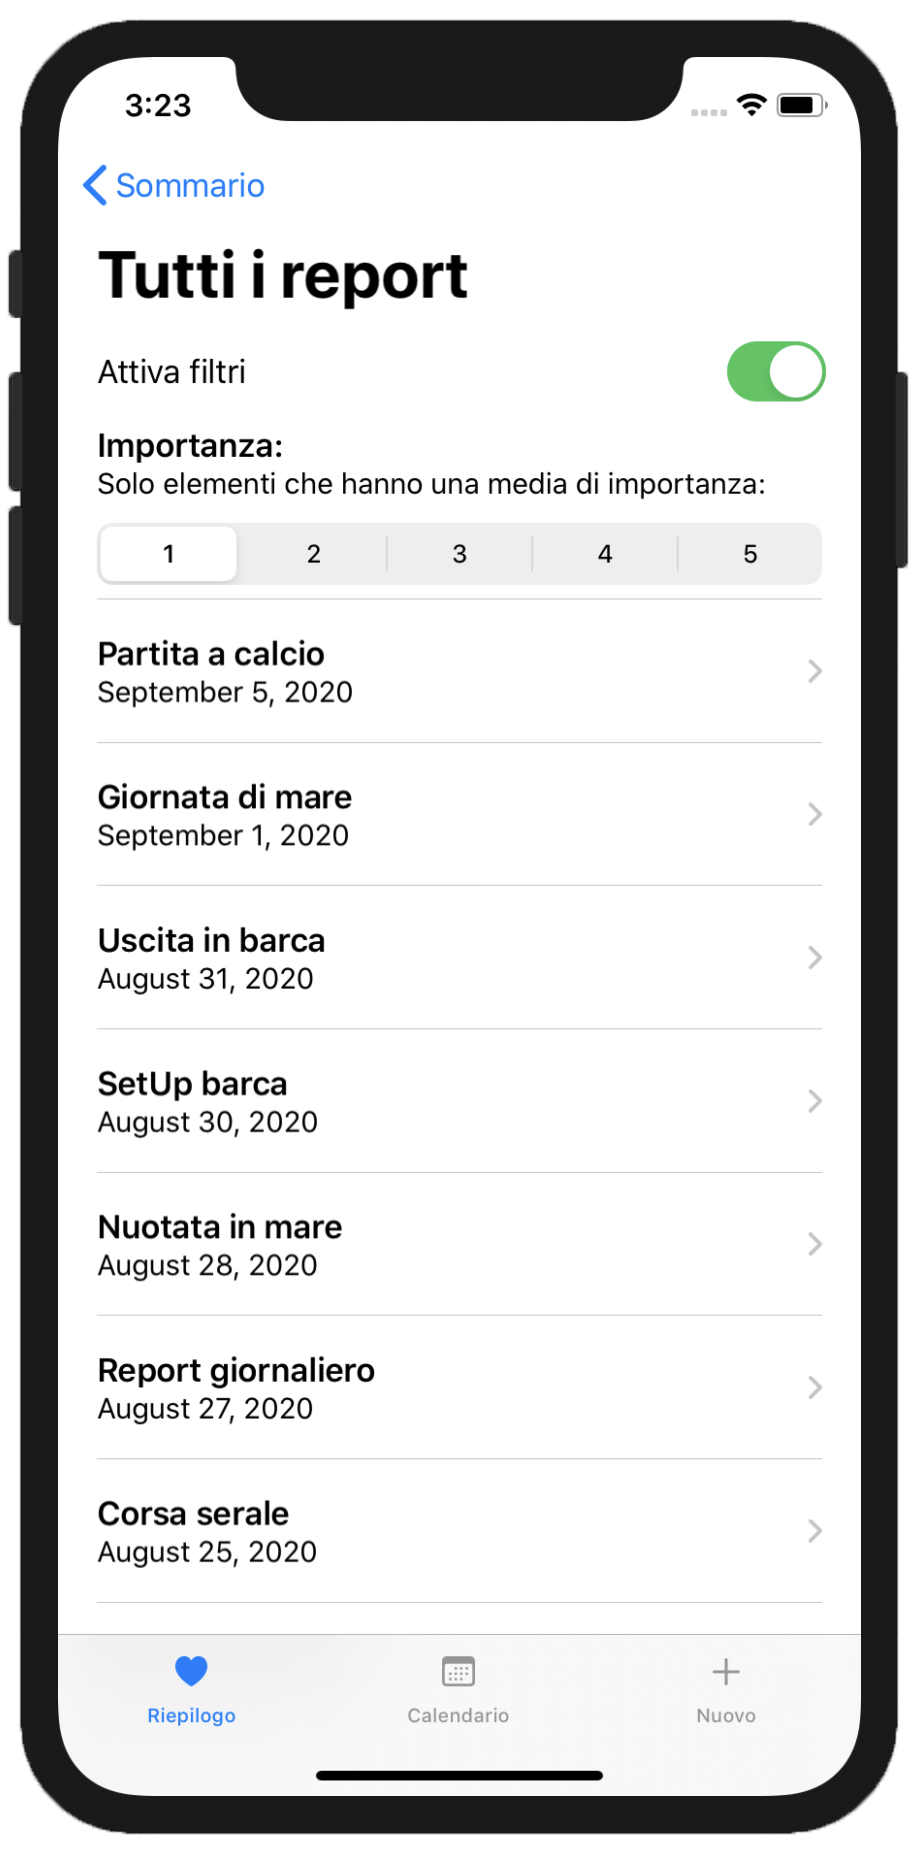
\includegraphics[width=.3\textwidth]{img/tutti2.png}\hfill
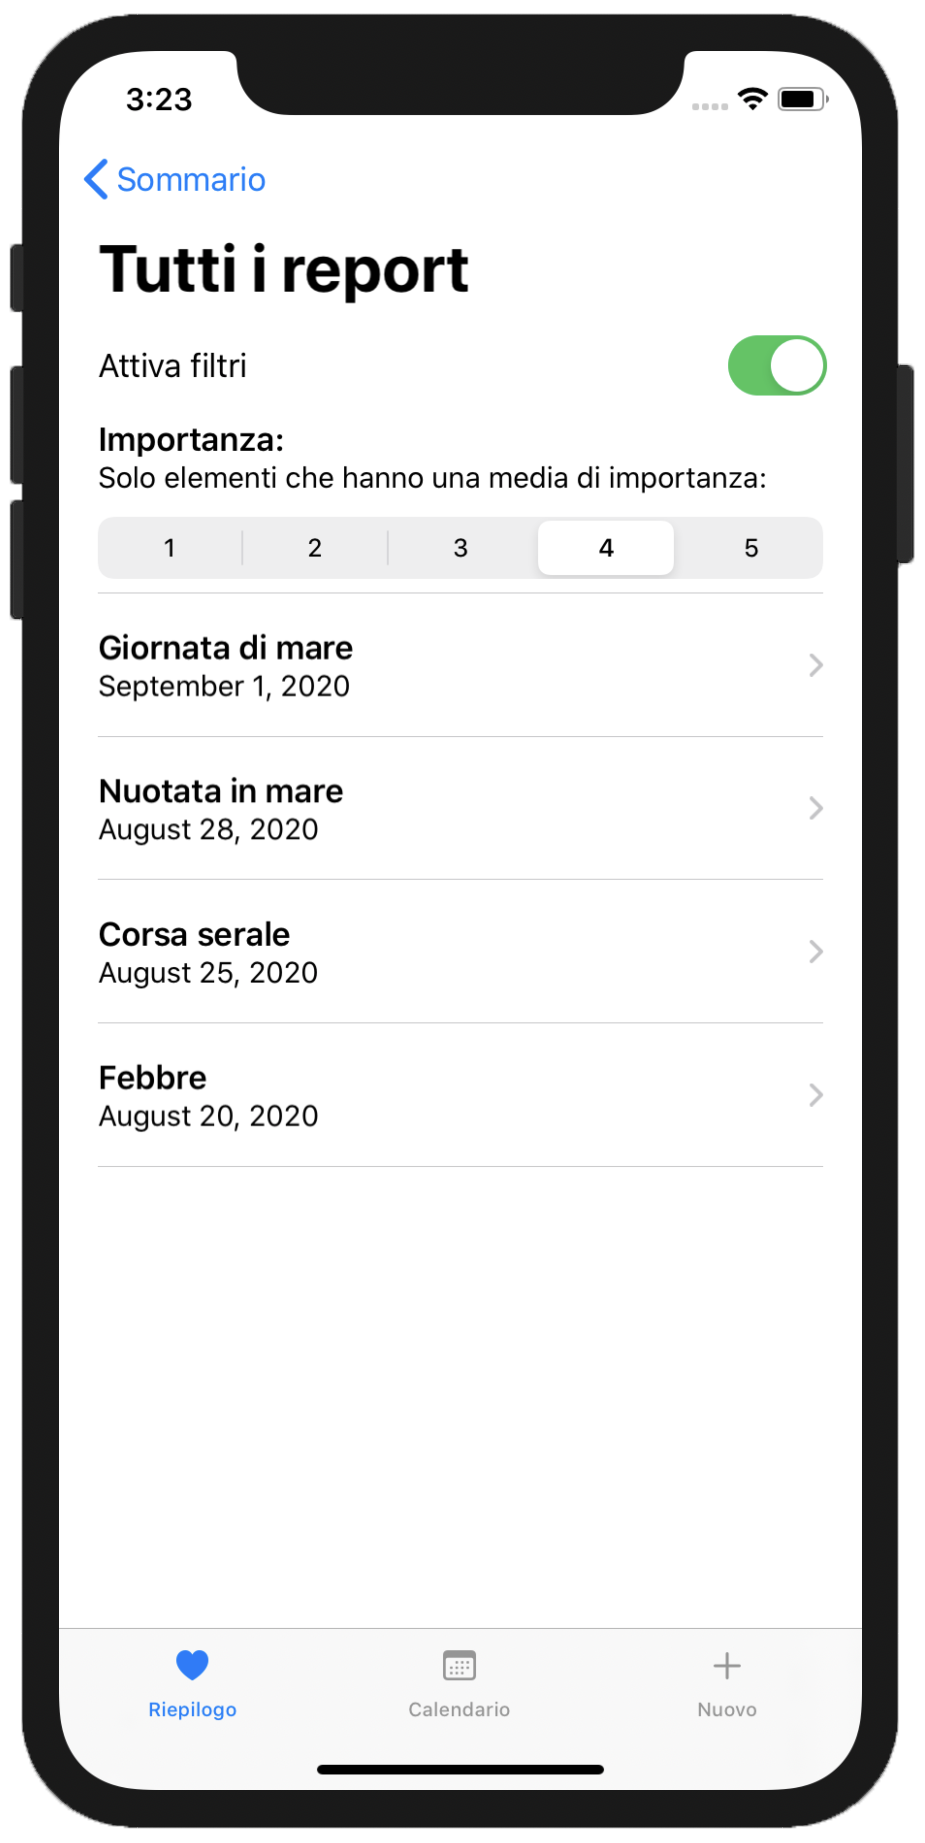
\includegraphics[width=.3\textwidth]{img/tutti3.png}

\caption{Grafici con valori}
\label{fig:figure3}

\end{figure}

%----------------------------------------------------------------------------------------
%	Calendario
%----------------------------------------------------------------------------------------

\newpage
\section{Calendario}

In riepilogo vengono generati i grafici relativi ai dati inseriti giorno per giorno inoltre è presenta una lista dove si possono consultare tutti i Report. Se non è presente nessun dato viene caricata una schermata iniziale di benvenuto. 

\begin{figure}[htp]

\centering
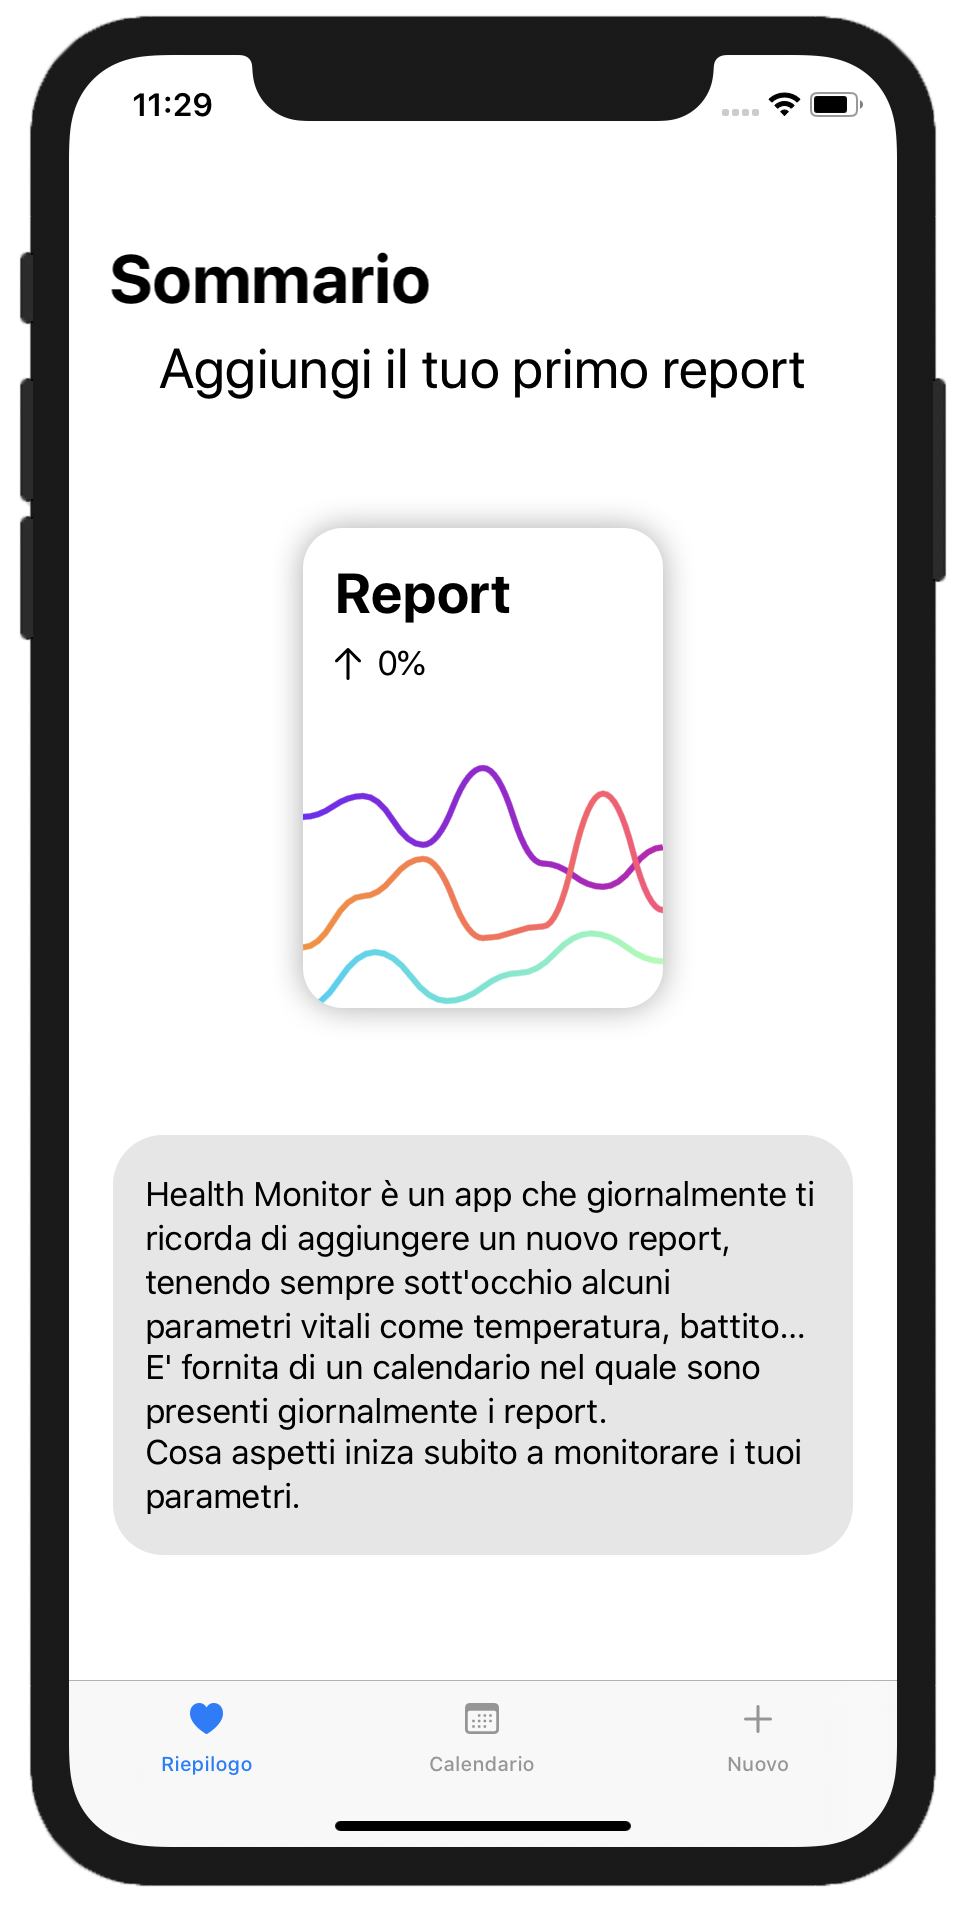
\includegraphics[width=.3\textwidth]{img/riepilogo_iniziale.png}

\caption{Schermata di benvenuto}
\label{fig:figure3}
\end{figure}

\subsection{Grafici}

Quando si inseriscono i dati, si iniziano a generare 4 grafici uno per ogni valore presente nel Report.\\
I grafici generati usando un pacchetto Swift \textbf{\textit{"SwiftUICharts"}}


%----------------------------------------------------------------------------------------
%	Nuovo
%----------------------------------------------------------------------------------------

\newpage
\section{Nuovo}

In riepilogo vengono generati i grafici relativi ai dati inseriti giorno per giorno inoltre è presenta una lista dove si possono consultare tutti i Report. Se non è presente nessun dato viene caricata una schermata iniziale di benvenuto. 

\begin{figure}[htp]

\centering
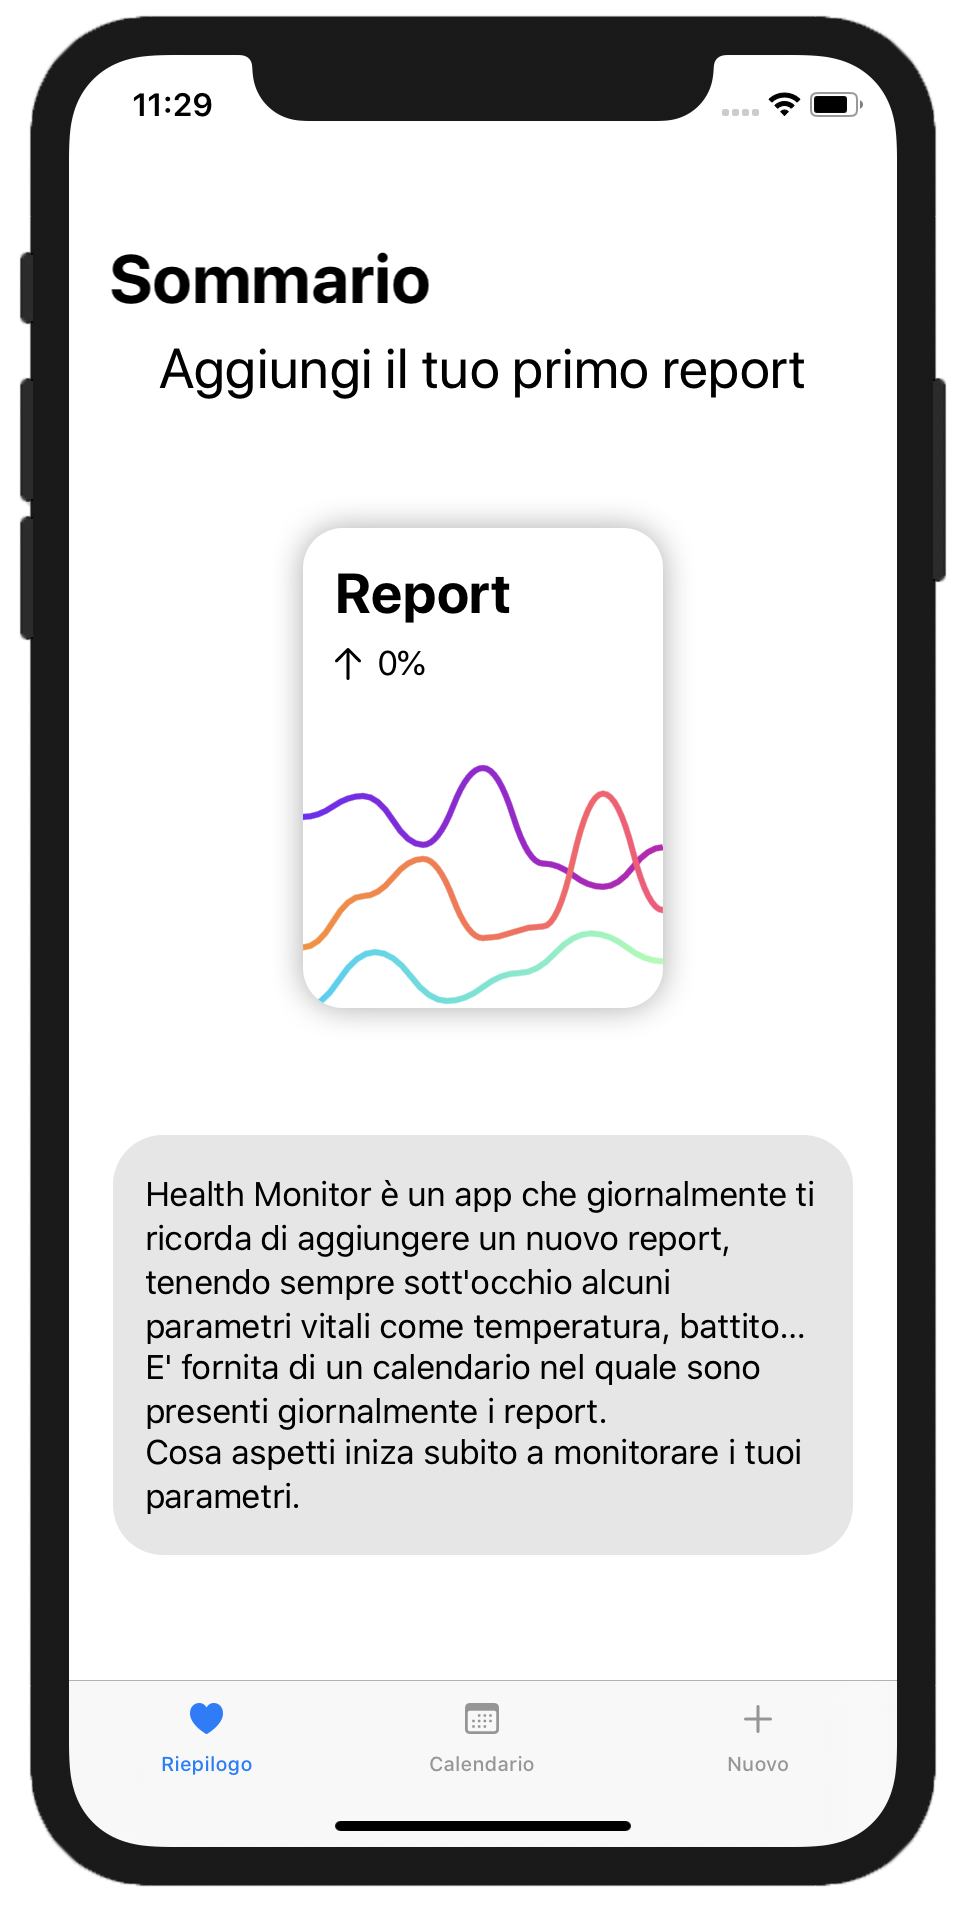
\includegraphics[width=.3\textwidth]{img/riepilogo_iniziale.png}

\caption{Schermata di benvenuto}
\label{fig:figure3}
\end{figure}

\subsection{Grafici}

Quando si inseriscono i dati, si iniziano a generare 4 grafici uno per ogni valore presente nel Report.\\
I grafici generati usando un pacchetto Swift \textbf{\textit{"SwiftUICharts"}}






%----------------------------------------------------------------------------------------
%	BIBLIOGRAPHY
%----------------------------------------------------------------------------------------

\bibliographystyle{apalike}

\bibliography{sample}

%----------------------------------------------------------------------------------------


\end{document}